
%=============================================================================
% 相变理论
%=============================================================================

相变（phase transition）是物理学中最迷人的现象之一。当系统的温度、压强或其他控制参数发生变化时，系统的宏观性质可能发生突变，这就是相变。水结冰、铁磁体失去磁性、超导体的出现，都是相变的例子。在 AdS/CFT 对偶中，相变同样扮演着重要角色：引力系统中的相变（如霍金-佩奇相变）对应于边界场论中的相变（如禁闭/解禁闭相变）\cite{Witten1998b}。本节将系统地介绍相变理论的基本概念，包括相变的分类、朗道理论、临界现象和全息相变。

\section{相变的分类}

相变可以按照不同的标准进行分类。分类的核心在于找到能够刻画相变本质特征的物理量，从而建立系统的分类框架。

\subsection{Ehrenfest 分类：基于自由能导数的不连续性}

\begin{note}
Ehrenfest 于 1933 年提出了最早的相变分类方案，其核心思想是：相变的阶数由自由能在相变点处第一个不连续的导数阶数决定。这一分类方法将所有相变纳入统一的数学框架。
\end{note}

设自由能为 $G(T, p)$，其 $n$ 阶导数为：
\begin{equation}
    G^{(n)} = \frac{\partial^n G}{\partial T^n}.
\end{equation}

\begin{definition}[$n$ 阶相变]
设热力学势 $G(T,p)$ 在相变点 $T_c$ 处满足：
\begin{itemize}
    \item $G^{(k)}$ 在 $T_c$ 处连续，对所有 $k \leq n-1$；
    \item $G^{(n)}$ 在 $T_c$ 处不连续。
\end{itemize}
则称该相变为 $n$ \textbf{阶相变}。
\end{definition}

在实际物理系统中，最常见的是一阶和二阶相变。下面我们分别详细讨论。

\begin{property}[一阶相变的特征]
一阶相变中，自由能的一阶导数不连续，具体表现为：
\begin{enumerate}
    \item 熵 $S = -\partial G/\partial T$ 不连续，产生潜热 $\Delta Q = T \Delta S$；
    \item 体积 $V = \partial G/\partial p$ 不连续，产生体积跳变 $\Delta V$；
    \item 在相变点处，两相的化学势相等 $\mu_1 = \mu_2$，但熵和体积不同，因此两相可以共存。
\end{enumerate}
\end{property}

\begin{property}[二阶相变的特征]
二阶相变中，自由能的一阶导数连续，但二阶导数不连续或发散，具体表现为：
\begin{enumerate}
    \item 热容 $C_p = -T \partial^2 G/\partial T^2$ 不连续或发散；
    \item 压缩率 $\kappa_T = -V^{-1} \partial V/\partial p$ 不连续或发散；
    \item 磁化率 $\chi_T$ 不连续或发散。
\end{enumerate}
序参量在临界点处连续变化，但其涨落变得长程相关。
\end{property}

表 \ref{tab:phase_transition_comparison} 总结了一阶相变和二阶相变的主要区别。

\begin{table}[htbp]
\centering
\begin{tabular}{|l|c|c|}
\hline
\textbf{特征} & \textbf{一阶相变} & \textbf{二阶相变} \\
\hline
自由能一阶导数 & 不连续 & 连续 \\
\hline
潜热 & 非零 & 零 \\
\hline
体积变化 & 突变 & 连续 \\
\hline
序参量 & 不连续跳变 & 连续变化 \\
\hline
临界涨落 & 弱 & 强 \\
\hline
两相共存 & 是 & 否 \\
\hline
\end{tabular}
\caption{一阶相变和二阶相变的主要区别。}
\label{tab:phase_transition_comparison}
\end{table}

\subsection{现代分类：一级相变与连续相变}

现代物理学中，Ehrenfest 分类被进一步简化为两大类：

\begin{definition}[一级相变]
自由能的一阶导数不连续，具有潜热和体积跳变。一级相变通常通过成核和生长机制发生，系统存在亚稳态（过冷或过热），并伴随滞后现象。
\end{definition}

\begin{definition}[连续相变]
自由能的一阶导数连续，但高阶导数在临界点处发散。连续相变的标志性特征是临界现象：关联长度发散、临界涨落、标度律和普适性。连续相变不涉及潜热和两相共存，序参量在临界点处连续趋于零。
\end{definition}

\begin{definition}[临界点]
连续相变的终点称为\textbf{临界点}。在临界点处，关联长度 $\xi \to \infty$，系统表现出尺度不变性，这使得临界行为可以用共形场论来描述。
\end{definition}

\begin{example}
水的液-气临界点位于 $T_c = 647\,\mathrm{K}$，$p_c = 22.1\,\mathrm{MPa}$。在临界点处，液相和气相的密度差趋于零，关联长度发散，临界乳光现象出现。
\end{example}

\subsection{量子相变}

\begin{remark}
热力学相变由热涨落驱动，在有限温度下发生。除此之外，还存在一类在绝对零度下发生的相变，称为量子相变（quantum phase transition）。量子相变由量子涨落驱动，通过改变非热力学参数（如磁场、压力或掺杂浓度）来实现。
\end{remark}

\begin{definition}[量子相变]
在绝对零度 $T = 0$ 下，通过调节非热力学控制参数 $g$（如磁场、压力、掺杂浓度），系统基态性质发生突变的现象称为\textbf{量子相变}。量子相变的临界点 $g = g_c$ 称为量子临界点。
\end{definition}

量子相变的分类框架与热力学相变类似，但有其独特之处。在量子相变中，$d$ 维量子系统的临界行为等价于 $d+z$ 维经典系统的临界行为，其中 $z$ 是动力学临界指数。

\begin{theorem}[量子-经典映射]
$d$ 维量子系统的临界行为等价于 $d+z$ 维经典系统的临界行为，其中 $z$ 是动力学临界指数。具体地，量子系统的关联长度 $\xi$ 和关联时间 $\tau$ 满足：
\begin{equation}
    \tau \sim \xi^z,
\end{equation}
有效空间维度为 $d_{\text{eff}} = d + z$。
\end{theorem}

\begin{remark}
量子相变的临界点处出现量子临界区域，在有限温度下展现出非费米液体行为。这在高温超导体和重费米子系统中具有重要意义。
\end{remark}

\subsection{拓扑相变}

朗道相变理论的核心是对称性破缺：相变由序参量的出现来表征，不同相由对称性来区分。然而，近年来发现了一类无法用对称性破缺描述的相变——拓扑相变（topological phase transition）。

\begin{definition}[拓扑相变]
拓扑相变的分类不依赖于序参量和对称性，而是由拓扑不变量来表征。拓扑不变量是定义在动量空间中的全局量，不能通过局域的微扰连续改变。当系统的参数跨越拓扑相变点时，拓扑不变量发生跳变，对应的边界态出现或消失。
\end{definition}

拓扑相变的理论框架基于纤维丛理论和 K-理论。对于能带系统，拓扑不变量可以从 Berry 联络和 Berry 曲率导出。

\begin{theorem}[陈数公式]
对于二维能带系统，第 $n$ 条能带的陈数定义为：
\begin{equation}
    C_n = \frac{1}{2\pi} \int_{\text{BZ}} F^{(n)}_{xy} \, dk_x dk_y,
\end{equation}
其中 $F^{(n)}_{xy} = \partial_{k_x} A^{(n)}_y - \partial_{k_y} A^{(n)}_x$ 是第 $n$ 条能带的 Berry 曲率，$A^{(n)}_i = i\langle u_n(\mathbf{k}) | \partial_{k_i} | u_n(\mathbf{k}) \rangle$ 是 Berry 联络，$|u_n(\mathbf{k})\rangle$ 是 Bloch 波函数。
\end{theorem}

\begin{proof}
Berry 曲率 $F^{(n)}_{xy}$ 是定义在 Brillouin 区上的曲率 2-形式。由于 Brillouin 区是紧致流形（二维环面 $T^2$），陈数是 Berry 曲率在 Brillouin 区上的积分除以 $2\pi$。陈数是整数值的拓扑不变量，其整数性来源于 Berry 联络的规范不变性。具体地，利用 Stokes 定理和 Bloch 波函数的周期性边界条件，可以证明该积分必为整数。
\end{proof}

\begin{example}
量子霍尔效应中，二维电子气的霍尔电导为 $\sigma_{xy} = C e^2/h$，其中 $C$ 是陈数。陈数的跳变对应于拓扑相变，此时能隙关闭并重新打开。
\end{example}

\subsection{相变分类的统一视角}

\begin{remark}
从更深层次看，相变的分类反映了系统自由度之间的关联方式。一级相变中，系统在两个局域极小值之间跳跃；连续相变中，系统在临界点处表现出长程关联和尺度不变性；量子相变中，量子纠缠取代热涨落成为驱动机制；拓扑相变中，全局的拓扑性质取代局域的序参量成为分类依据。
\end{remark}

在 AdS/CFT 对偶中，不同类型的相变对应于体空间中不同类型的几何变化。一级相变对应于几何的不连续跳变，连续相变对应于几何的连续形变，这为理解强耦合系统中的相变提供了统一的几何框架。

\section{朗道理论}

朗道理论是研究相变的经典理论，由朗道（Landau）于 1937 年提出 \cite{Landau1937}。朗道理论的核心思想是：相变可以用一个序参量（order parameter）$m$ 来描述，自由能可以展开为序参量的幂级数。

\subsection{序参量的概念}

\begin{note}
在描述相变之前，我们需要找到一个能够区分不同相的物理量。这个量在对称相中应该为零，在对称性破缺相中应该非零。这就是序参量的物理意义。
\end{note}

\begin{definition}[序参量]
序参量是描述系统有序程度的物理量。在不同的物理系统中，序参量有不同的含义：
\begin{itemize}
    \item \textbf{铁磁体}：序参量是磁化强度 $m$，描述磁矩的集体取向
    \item \textbf{液-气相变}：序参量是密度差 $\rho_l - \rho_g$，描述液相和气相的密度差异
    \item \textbf{超导体}：序参量是库珀对的凝聚波函数 $\psi$，描述超导电子的集体行为
    \item \textbf{超流体}：序参量是玻色-爱因斯坦凝聚的波函数 $\psi$
    \item \textbf{向列相液晶}：序参量是张量 $Q_{ij}$，描述分子取向的有序程度
\end{itemize}
序参量的选择不是唯一的，但好的序参量应该满足：在对称相中为零，在对称性破缺相中非零。
\end{definition}

\begin{remark}
在 AdS/CFT 对偶中，序参量可以由体空间中的场来表示。例如，全息超导体的序参量对应于体空间中的复标量场在边界上的渐近值。
\end{remark}

\subsection{自由能展开}

\begin{note}
朗道理论的基本假设是：在临界点附近，自由能可以解析地展开为序参量的幂级数。这个假设的物理基础是：在临界点附近，序参量是一个小量，高阶项可以忽略。
\end{note}

\begin{definition}[朗道自由能]\label{def:landau_free_energy}
考虑一个具有 $Z_2$ 对称性（$m \to -m$）的系统，如铁磁体。朗道理论将自由能密度展开为序参量的幂级数：
\begin{equation}
    \mathcal{L}[m; T, H] = \mathcal{L}_0 + \frac{1}{2}a m^2 + \frac{1}{4}b m^4 + \cdots - mH,
\end{equation}
其中 $a = a_0(T - T_c)$，$a_0 > 0$，$b > 0$，$H$ 是外场。
\end{definition}

\begin{remark}
各项的物理意义：
\begin{itemize}
    \item $\mathcal{L}_0$：对称相的自由能密度，与序参量无关
    \item $\frac{1}{2}a m^2$：二次项，系数 $a$ 的符号决定相变行为
    \item $\frac{1}{4}b m^4$：四次项，保证自由能有下界，$b > 0$
    \item $-mH$：外场与序参量的耦合
\end{itemize}
为什么只保留偶数次幂？这是因为系统具有 $Z_2$ 对称性 $m \to -m$，自由能必须是 $m$ 的偶函数。如果系统具有更高的对称性（如 $O(N)$ 对称性），自由能的形式会更复杂。
\end{remark}

\subsection{平衡条件与相变}

\begin{theorem}[朗道平衡条件]\label{thm:landau_equilibrium}
在无外场（$H = 0$）的情况下，朗道自由能的极值条件给出平衡态序参量满足：
\begin{equation}
    m(a + b m^2) = 0.
\end{equation}
\end{theorem}

\begin{proof}
平衡态由自由能的极值条件决定：
\begin{equation}
    \frac{\partial \mathcal{L}}{\partial m} = a m + b m^3 - H = 0.
\end{equation}
令 $H = 0$，得到：
\begin{equation}
    a m + b m^3 = m(a + b m^2) = 0.
\end{equation}
这个方程有两个解：
\begin{enumerate}
    \item $m = 0$：对称解
    \item $m^2 = -a/b$：对称性破缺解，当且仅当 $a < 0$ 时存在
\end{enumerate}

当 $T > T_c$ 时，$a = a_0(T - T_c) > 0$，只有 $m = 0$ 是稳定解（对应自由能的极小值），系统处于对称相。

当 $T < T_c$ 时，$a < 0$，$m = 0$ 变为不稳定解（对应自由能的极大值）。稳定解为：
\begin{equation}
    m_0 = \pm \sqrt{-\frac{a}{b}} = \pm \sqrt{\frac{a_0(T_c - T)}{b}}.
\end{equation}
这可以通过检验二阶导数来确认：
\begin{equation}
    \frac{\partial^2 \mathcal{L}}{\partial m^2}\bigg|_{m=m_0} = a + 3b m_0^2 = a + 3b \cdot \left(-\frac{a}{b}\right) = -2a > 0,
\end{equation}
因此 $m = m_0$ 确实是极小值点。
\end{proof}

图 \ref{fig:Landau} 展示了朗道势在不同温度下的形状。

\begin{figure}[htbp]
\centering
\begin{subfigure}[b]{0.45\textwidth}
\centering
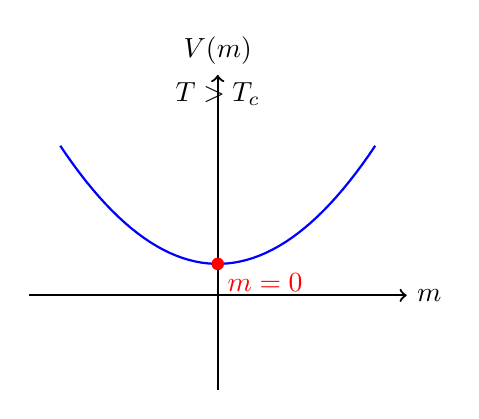
\begin{tikzpicture}[scale=0.8]
    \draw[thick, ->] (-3,0) -- (3,0) node[right] {$m$};
    \draw[thick, ->] (0,-1.5) -- (0,3.5) node[above] {$V(m)$};
    
    % 绘制 T > Tc 的势 - 单势阱
    \draw[thick, blue, domain=-2.5:2.5, samples=50] plot (\x, {0.5 + 0.3*\x*\x});
    
    % 标注最小值点 - 准确在曲线上
    \fill[red] (0,0.5) circle (0.1) node[below right] {$m=0$};
    
    \node at (0,3.2) {$T > T_c$};
\end{tikzpicture}
\end{subfigure}
\hfill
\begin{subfigure}[b]{0.45\textwidth}
\centering
\begin{tikzpicture}[scale=0.8]
    \draw[thick, ->] (-3,0) -- (3,0) node[right] {$m$};
    \draw[thick, ->] (0,-1.5) -- (0,3.5) node[above] {$V(m)$};
    
    % 绘制 T < Tc 的势 - 双势阱
    \draw[thick, blue, domain=-2.8:2.8, samples=100] plot (\x, {0.5 - 0.5*\x*\x + 0.05*\x*\x*\x*\x});
    
    % 标注最小值点 - 准确在曲线上
    \fill[red] (-2.236,-0.75) circle (0.1) node[below] {$-m_0$};
    \fill[red] (2.236,-0.75) circle (0.1) node[below] {$m_0$};
    
    % 标注不稳定点
    \fill[green] (0,0.5) circle (0.1) node[above right] {$m=0$ (不稳定)};
    
    % 添加虚线辅助
    \draw[dashed, gray] (-2.236,-0.75) -- (-2.236,0);
    \draw[dashed, gray] (2.236,-0.75) -- (2.236,0);
    
    \node at (0,3.2) {$T < T_c$};
\end{tikzpicture}
\end{subfigure}
\caption{朗道势示意图。左图：$T > T_c$ 时，势在 $m=0$ 处有唯一最小值。右图：$T < T_c$ 时，势在 $m = \pm m_0$ 处有两个最小值，发生自发对称性破缺。}
\label{fig:Landau}
\end{figure}

\subsection{平衡态自由能}

将平衡解代入自由能表达式，得到平衡态自由能。

\begin{theorem}[平衡态自由能]
在对称相（$T > T_c$）中，平衡态自由能为：
\begin{equation}
    \mathcal{L}_{\text{eq}} = \mathcal{L}_0.
\end{equation}
在对称性破缺相（$T < T_c$）中，平衡态自由能为：
\begin{equation}
    \mathcal{L}_{\text{eq}} = \mathcal{L}_0 - \frac{a^2}{4b} = \mathcal{L}_0 - \frac{a_0^2(T_c - T)^2}{4b}.
\end{equation}
\end{theorem}

\begin{proof}
在对称相中，$m = 0$，直接代入朗道自由能得 $\mathcal{L}_{\text{eq}} = \mathcal{L}_0$。

在对称性破缺相中，$m = m_0 = \sqrt{-a/b}$，代入朗道自由能：
\begin{align}
    \mathcal{L}_{\text{eq}} &= \mathcal{L}_0 + \frac{1}{2}a m_0^2 + \frac{1}{4}b m_0^4 \nonumber \\
    &= \mathcal{L}_0 + \frac{1}{2}a \left(-\frac{a}{b}\right) + \frac{1}{4}b \left(-\frac{a}{b}\right)^2 \nonumber \\
    &= \mathcal{L}_0 - \frac{a^2}{2b} + \frac{a^2}{4b} \nonumber \\
    &= \mathcal{L}_0 - \frac{a^2}{4b}.
\end{align}
将 $a = a_0(T - T_c)$ 代入，得到 $\mathcal{L}_{\text{eq}} = \mathcal{L}_0 - a_0^2(T_c - T)^2/(4b)$。
\end{proof}

\begin{note}
自由能在相变点处连续，但其导数不连续。具体来说：
\begin{itemize}
    \item 自由能的一阶导数（熵）在相变点处连续，因此这是二阶相变
    \item 自由能的二阶导数（热容）在相变点处不连续
\end{itemize}
这正是二阶相变的特征。
\end{note}

\subsection{响应函数}

朗道理论还可以计算系统的响应函数。

\begin{definition}[磁化率]
磁化率描述系统对外场的线性响应，定义为：
\begin{equation}
    \chi_T = \frac{\partial m}{\partial H}\bigg|_{H=0}.
\end{equation}
\end{definition}

\begin{theorem}[朗道理论的磁化率]
在对称相（$T > T_c$）中：
\begin{equation}
    \chi_T = \frac{1}{a} = \frac{1}{a_0(T - T_c)}, \quad T > T_c.
\end{equation}
在对称性破缺相（$T < T_c$）中：
\begin{equation}
    \chi_T = \frac{1}{2|a|} = \frac{1}{2a_0(T_c - T)}, \quad T < T_c.
\end{equation}
\end{theorem}

\begin{proof}
对平衡条件 $am + bm^3 = H$ 关于 $H$ 求导：
\begin{equation}
    a \frac{\partial m}{\partial H} + 3b m^2 \frac{\partial m}{\partial H} = 1,
\end{equation}
即：
\begin{equation}
    \chi_T = \frac{\partial m}{\partial H} = \frac{1}{a + 3b m^2}.
\end{equation}

在对称相中，$m = 0$，因此 $\chi_T = 1/a$。由于 $a = a_0(T - T_c)$，得到 $\chi_T = 1/[a_0(T - T_c)]$。

在对称性破缺相中，$m_0^2 = -a/b$，因此：
\begin{equation}
    \chi_T = \frac{1}{a + 3b(-a/b)} = \frac{1}{a - 3a} = \frac{1}{-2a} = \frac{1}{2|a|}.
\end{equation}
\end{proof}

\begin{remark}
磁化率在临界点处发散，发散指数为 $\gamma = 1$。这表明系统在临界点处对外场极其敏感，微小的外场可以引起巨大的响应。这是临界现象的重要特征之一。
\end{remark}

\begin{definition}[热容]
热容描述系统对温度变化的响应，定义为：
\begin{equation}
    C = -T \frac{\partial^2 \mathcal{L}_{\text{eq}}}{\partial T^2}.
\end{equation}
\end{definition}

\begin{theorem}[朗道理论的热容跳变]
在相变点处，热容发生跳变，跳变量为：
\begin{equation}
    \Delta C = \frac{a_0^2 T_c}{2b}.
\end{equation}
\end{theorem}

\begin{proof}
在对称相中，$\mathcal{L}_{\text{eq}} = \mathcal{L}_0$，热容为 $C = C_0$。

在对称性破缺相中，$\mathcal{L}_{\text{eq}} = \mathcal{L}_0 - a_0^2(T_c - T)^2/(4b)$，对 $T$ 求二阶导数：
\begin{equation}
    \frac{\partial^2 \mathcal{L}_{\text{eq}}}{\partial T^2} = \frac{\partial^2 \mathcal{L}_0}{\partial T^2} - \frac{a_0^2}{4b} \cdot 2 = \frac{\partial^2 \mathcal{L}_0}{\partial T^2} - \frac{a_0^2}{2b}.
\end{equation}
因此热容为：
\begin{equation}
    C = C_0 + \frac{a_0^2 T_c}{2b}, \quad T < T_c.
\end{equation}
跳变量为 $\Delta C = a_0^2 T_c / (2b)$。
\end{proof}

\subsection{自发对称性破缺}

\begin{note}
当 $T < T_c$ 时，系统必须选择一个最小值，$m = +m_0$ 或 $m = -m_0$。这个选择破坏了 $Z_2$ 对称性，称为自发对称性破缺。在铁磁体中，这对应于磁化强度指向某个特定方向。
\end{note}

\begin{definition}[自发对称性破缺]
当系统哈密顿量具有某种对称性，但基态不具有该对称性时，称为\textbf{自发对称性破缺}。其关键特征为：
\begin{enumerate}
    \item \textbf{简并性}：存在多个等价的基态，它们通过对称性变换相联系
    \item \textbf{选择性}：系统必须选择其中一个基态，这个选择是随机的
    \item \textbf{长程有序}：序参量在整个系统中具有非零期望值
\end{enumerate}
\end{definition}

\begin{remark}
在外场 $H \neq 0$ 的情况下，对称性被显式破缺，系统只有一个最小值。当 $H \to 0$ 时，系统会选择哪个最小值取决于 $H$ 的符号。自发对称性破缺与显式对称性破缺的本质区别在于：前者是系统自身的集体行为，后者是由外部因素导致的。
\end{remark}

\subsection{临界指数}

\begin{note}
临界指数是描述物理量在临界点附近奇异行为的幂律指数。朗道理论作为平均场理论，给出了临界指数的解析值。
\end{note}

\begin{property}[朗道理论的临界指数]
朗道理论给出的临界指数为：
\begin{align}
    m &\propto (T_c - T)^{1/2}, \quad \beta = 1/2, \\
    \chi_T &\propto |T - T_c|^{-1}, \quad \gamma = 1, \\
    C &\propto |T - T_c|^{0}, \quad \alpha = 0.
\end{align}
这些临界指数与平均场理论（mean-field theory）的结果一致。事实上，朗道理论就是平均场理论的一种表述方式。
\end{property}

\begin{theorem}[Rushbrooke 标度律]
临界指数之间满足标度关系：
\begin{equation}
    \alpha + 2\beta + \gamma = 2.
\end{equation}
\end{theorem}

\begin{proof}
朗道理论的结果满足这个标度律：$0 + 2 \times (1/2) + 1 = 2$。一般地，标度律源于自由能在临界点附近的齐次性质。设自由能密度具有标度形式 $f(t, H) = b^{-d} f(b^{y_t} t, b^{y_h} H)$，其中 $t = (T - T_c)/T_c$，$b$ 是标度因子，$y_t$ 和 $y_h$ 是标度维数。选择 $b = |t|^{-1/y_t}$，得到：
\begin{equation}
    f(t, H) = |t|^{d/y_t} f_\pm\left(\frac{H}{|t|^{y_h/y_t}}\right).
\end{equation}
从热容的定义 $C \sim \partial^2 f/\partial t^2$，得到 $\alpha = 2 - d/y_t$。从序参量的定义 $m \sim \partial f/\partial H$，得到 $\beta = (d - y_h)/y_t$。从磁化率的定义 $\chi \sim \partial^2 f/\partial H^2$，得到 $\gamma = (2y_h - d)/y_t$。将这三个关系相加：
\begin{equation}
    \alpha + 2\beta + \gamma = \left(2 - \frac{d}{y_t}\right) + 2\cdot\frac{d - y_h}{y_t} + \frac{2y_h - d}{y_t} = 2.
\end{equation}
\end{proof}

\subsection{朗道理论的适用范围}

\begin{note}
朗道理论是一个平均场理论，它忽略了涨落的影响。理解其适用条件对于正确应用该理论至关重要。
\end{note}

\begin{theorem}[上临界维度]
朗道理论的适用条件为：
\begin{enumerate}
    \item \textbf{空间维度足够高}：当 $d > d_c = 4$ 时，朗道理论是精确的。$d_c = 4$ 称为上临界维度。
    \item \textbf{关联长度足够大}：当关联长度远大于微观尺度时，涨落的影响可以忽略。
    \item \textbf{序参量梯度小}：当序参量在空间中变化缓慢时，梯度项可以忽略。
\end{enumerate}
\end{theorem}

\begin{remark}
当这些条件不满足时，涨落变得重要，朗道理论失效。此时需要使用重正化群理论来处理临界现象。值得注意的是，在 AdS/CFT 对偶中，强耦合极限下涨落被抑制，平均场理论（即朗道理论）往往变得精确。这解释了为什么全息超导体的临界指数与平均场结果一致。
\end{remark}

\subsection{推广到高维序参量}

朗道理论可以推广到更复杂的对称性。对于具有 $O(N)$ 对称性的系统，序参量是一个 $N$ 维矢量 $\mathbf{m} = (m_1, m_2, \ldots, m_N)$。

\begin{definition}[$O(N)$ 朗道自由能]
$O(N)$ 对称系统的朗道自由能为：
\begin{equation}
    \mathcal{L}[\mathbf{m}] = \mathcal{L}_0 + \frac{1}{2}a |\mathbf{m}|^2 + \frac{1}{4}b |\mathbf{m}|^4.
\end{equation}
其中 $|\mathbf{m}|^2 = \sum_{i=1}^N m_i^2$。
\end{definition}

\begin{example}
这个模型描述了许多重要的物理系统：
\begin{itemize}
    \item $N = 1$：伊辛模型，描述铁磁体
    \item $N = 2$：XY 模型，描述超流体和超导体
    \item $N = 3$：海森堡模型，描述各向同性铁磁体
\end{itemize}
\end{example}

\begin{theorem}[Goldstone 定理]
对于 $N \geq 2$ 的情况，$O(N)$ 对称性自发破缺为 $O(N-1)$ 时，会出现 $N-1$ 个无质量的 Goldstone 玻色子。
\end{theorem}

\begin{proof}
当 $T < T_c$ 时，序参量选择一个方向 $\mathbf{m}_0 = (m_0, 0, \ldots, 0)$，$O(N)$ 对称性破缺为 $O(N-1)$。在破缺方向上，序参量可以在简并的基态之间连续变化。这些简并基态构成一个 $N-1$ 维的球面 $S^{N-1}$，对应的激发模式是无质量的。具体地，将序参量写为 $\mathbf{m} = (m_0 + \sigma, \pi_1, \ldots, \pi_{N-1})$，其中 $\sigma$ 是径向涨落（有质量），$\pi_i$ 是切向涨落（无质量 Goldstone 模式）。在长波极限下，Goldstone 模式的色散关系为 $\omega \propto k$，即线性色散。
\end{proof}

\subsection{不具有 $Z_2$ 对称性的情况}

\begin{note}
当系统不具有 $m \to -m$ 对称性时，自由能展开中可以存在奇数次幂项，相变行为会发生质的变化。
\end{note}

当系统不具有 $Z_2$ 对称性时，自由能展开中可以存在奇数次幂项。例如，对于液-气相变，自由能为：
\begin{equation}
    \mathcal{L}[m; T, H] = \frac{1}{2} a m^2 - \frac{1}{3} c m^3 + \frac{1}{4} b m^4 + \cdots - m H,
\end{equation}
其中 $m^3$ 项破坏了 $Z_2$ 对称性。

\begin{property}[一阶相变条件]
当 $c \neq 0$ 时，相变可以是一阶相变，具有以下特征：
\begin{enumerate}
    \item 序参量在相变点处不连续跳变
    \item 存在潜热和相变滞后
    \item 存在亚稳态（过冷或过热）
\end{enumerate}
\end{property}

\begin{remark}
这与具有 $Z_2$ 对称性的系统（如铁磁体）形成对比，后者在平均场理论中总是发生二阶相变。$m^3$ 项的存在使得自由能势从双势阱变为非对称势阱，导致一级相变行为。
\end{remark}

\subsection{相变的统计力学描述}

从统计力学的角度，相变可以通过配分函数来描述。

\begin{definition}[序参量的配分函数]
序参量的配分函数定义为：
\begin{equation}
    Z = \int \mathcal{D}m \, e^{-\beta \mathcal{F}[m; T, H]},
\end{equation}
其中 $\mathcal{F}[m; T, H]$ 是自由能泛函，$\beta = 1/(k_B T)$。
\end{definition}

\begin{remark}
在平均场近似下，忽略涨落，用鞍点近似：
\begin{equation}
    Z \simeq e^{-\beta F_{\text{on-shell}}(T, H)},
\end{equation}
其中 $F_{\text{on-shell}}$ 是在鞍点处的自由能。然而，在临界点附近，涨落变得重要，平均场理论失效。此时需要使用重正化群方法来处理临界现象。
\end{remark}

\section{临界现象}

在连续相变的临界点附近，系统展现出一系列普适的奇异行为，统称为临界现象。临界现象的理论框架基于三个核心概念：关联长度发散、标度律和普适性。

\subsection{临界点与关联长度}

\begin{note}
临界点是连续相变的终点，在该点处序参量连续趋于零。理解关联长度的发散是理解临界现象的关键。
\end{note}

\begin{definition}[关联函数与关联长度]
两点关联函数定义为：
\begin{equation}
    G(\mathbf{x}) = \langle \phi(\mathbf{x}) \phi(\mathbf{0}) \rangle - \langle \phi \rangle^2.
\end{equation}
在临界点附近，关联函数的衰减行为为：
\begin{equation}
    G(\mathbf{x}) \sim \frac{e^{-|\mathbf{x}|/\xi}}{|\mathbf{x}|^{d-2+\eta}},
\end{equation}
其中 $d$ 是空间维度，$\eta$ 是反常维数，$\xi$ 是关联长度。关联长度按幂律发散：
\begin{equation}
    \xi \propto |T - T_c|^{-\nu}.
\end{equation}
\end{definition}

\begin{remark}
关联长度的发散具有深远的物理后果。当 $\xi \to \infty$ 时，系统在所有尺度上都存在关联，微观细节变得不重要，系统表现出尺度不变性。这使得临界行为可以用共形场论来描述。在 AdS/CFT 对偶中，关联长度的发散对应于体空间中黑洞视界附近的几何奇异性。
\end{remark}

\subsection{临界指数的定义}

\begin{definition}[四个独立的临界指数]
定义约化温度 $t = (T - T_c)/T_c$，四个独立的临界指数定义为：
\begin{align}
    &\text{比热容：} & C &\propto |t|^{-\alpha}, \\
    &\text{序参量：} & m &\propto (-t)^{\beta} \quad (t < 0), \\
    &\text{磁化率：} & \chi_T &\propto |t|^{-\gamma}, \\
    &\text{临界等温线：} & m &\propto |H|^{1/\delta} \quad (t = 0).
\end{align}
\end{definition}

\begin{remark}
这四个指数并非完全独立。它们之间存在标度关系，这些标度关系源于自由能在临界点附近的齐次性质。
\end{remark}

\subsection{标度律}

\begin{theorem}[四大标度律]
临界指数之间满足以下标度关系：
\begin{enumerate}
    \item Rushbrooke 标度律：$\alpha + 2\beta + \gamma = 2$
    \item Widom 标度律：$\gamma = \beta(\delta - 1)$
    \item Fisher 标度律：$\gamma = \nu(2 - \eta)$
    \item Josephson 标度律：$\nu d = 2 - \alpha$
\end{enumerate}
\end{theorem}

\begin{proof}[标度律的推导]
这些标度律源于自由能在临界点附近的广义齐次性质。设自由能密度具有标度形式：
\begin{equation}
    f(t, H) = b^{-d} f(b^{y_t} t, b^{y_h} H),
\end{equation}
其中 $b$ 是任意标度因子，$y_t$ 和 $y_h$ 是热力学标度维数。

选择 $b = |t|^{-1/y_t}$，可以得到：
\begin{equation}
    f(t, H) = |t|^{d/y_t} f_{\pm}\left(\frac{H}{|t|^{y_h/y_t}}\right),
\end{equation}
其中 $f_{\pm}$ 是标度函数，$\pm$ 对应 $t > 0$ 和 $t < 0$。

从这个表达式可以推导出临界指数与标度维数的关系：
\begin{align}
    \alpha &= 2 - \frac{d}{y_t}, \\
    \beta &= \frac{d - y_h}{y_t}, \\
    \gamma &= \frac{2y_h - d}{y_t}, \\
    \delta &= \frac{y_h}{d - y_h}.
\end{align}
将这些关系代入各标度律，即可验证它们的正确性。
\end{proof}

\subsection{标度假设与标度函数}

\begin{definition}[标度假设]
标度假设（scaling hypothesis）是理解临界现象的关键假设。它假设在临界点附近，自由能密度是广义齐次函数：
\begin{equation}
    G(t, H) = b^{-d} G(b^{y_t} t, b^{y_h} H),
\end{equation}
其中 $b$ 是任意标度因子，$y_t$ 和 $y_h$ 是热力学标度维数。
\end{definition}

\begin{remark}
标度假设的物理基础是：在临界点附近，关联长度是唯一的特征长度，所有物理量的标度行为都由关联长度的发散决定。当 $b$ 取为关联长度 $\xi \sim |t|^{-\nu}$ 时，标度假设意味着自由能密度可以写为：
\begin{equation}
    f \sim \xi^{-d} \sim |t|^{\nu d}.
\end{equation}
这给出了 Josephson 标度律 $\alpha = 2 - \nu d$。
\end{remark}

\subsection{普适性}

\begin{definition}[普适性与普适类]
普适性（universality）是指不同的物理系统可能具有相同的临界指数，属于同一个普适类。普适类由两个因素唯一确定：
\begin{enumerate}
    \item \textbf{空间维度} $d$：维度越高，涨落的影响越小
    \item \textbf{序参量的对称性}：如 $Z_2$（伊辛）、$O(2)$（XY）、$O(3)$（海森堡）
\end{enumerate}
\end{definition}

\begin{remark}
普适性的物理根源在于关联长度的发散。当 $\xi \to \infty$ 时，微观细节被"冲刷掉"，只有长程行为（由对称性和维度决定）才重要。这使得截然不同的物理系统（如铁磁体和液体）可以具有相同的临界行为。
\end{remark}

\begin{example}
三维伊辛模型的临界指数为 $\alpha \approx 0.11$，$\beta \approx 0.33$，$\gamma \approx 1.24$，$\nu \approx 0.63$。这些指数描述了单轴铁磁体、液-气临界点和二元合金混合等完全不同的物理系统。
\end{example}

\subsection{临界现象的理论方法}

\begin{note}
临界现象的理论研究主要依赖以下三种方法，每种方法都有其独特的优势和适用范围。
\end{note}

临界现象的理论研究主要依赖以下方法：
\begin{itemize}
    \item \textbf{$\epsilon$ 展开}：在 $d = 4 - \epsilon$ 维中进行微扰展开，然后解析延拓到 $d = 3$
    \item \textbf{重正化群}：通过系统地积分掉短程涨落，研究耦合常数的流动
    \item \textbf{共形场论}：利用临界点处的尺度不变性和共形不变性
\end{itemize}

\begin{remark}
重正化群方法是理解临界现象最有力的工具。它不仅解释了普适性，还提供了计算临界指数的系统方法。在 AdS/CFT 对偶中，重正化群流对应于体空间中的径向演化，这为理解临界现象提供了新的几何视角。具体地，体空间的径向坐标 $r$ 对应于能量标度，从边界到体内部的演化对应于从紫外到红外的重正化群流。
\end{remark}

\section{金兹堡-朗道理论}

金兹堡-朗道理论（Ginzburg-Landau theory）是朗道理论的空间推广，由金兹堡和朗道于 1950 年提出 \cite{Ginzburg1950}，用于描述超导体等系统中的相变。与朗道理论不同，金兹堡-朗道理论考虑了序参量的空间变化，因此可以描述非均匀系统。

\subsection{物理动机}

\begin{note}
朗道理论假设序参量在空间中是均匀的，但在许多物理系统中，序参量会在空间中发生变化。例如，超导体中的序参量在超导-正常态界面上会发生空间变化。金兹堡-朗道理论通过引入序参量的梯度项来描述这种非均匀性。
\end{note}

\subsection{自由能泛函}

\begin{definition}[金兹堡-朗道自由能泛函]
金兹堡-朗道理论的自由能泛函为：
\begin{equation}
    F[\psi, \mathbf{A}] = \int d^3x \left[ \alpha|\psi|^2 + \frac{\beta}{2}|\psi|^4 + \gamma|(\nabla - ie\mathbf{A})\psi|^2 + \frac{1}{2\mu_0}(\nabla \times \mathbf{A})^2 \right],
\end{equation}
其中：
\begin{itemize}
    \item $\psi$ 是序参量（超导序参量），描述库珀对的凝聚
    \item $\mathbf{A}$ 是矢量势，描述电磁场
    \item $\alpha = a_0(T - T_c)$，当 $T < T_c$ 时 $\alpha < 0$
    \item $\beta > 0$ 是四次项系数
    \item $\gamma$ 是梯度项系数，描述序参量的空间变化
    \item $e$ 是电荷，$\mu_0$ 是真空磁导率
\end{itemize}
\end{definition}

\begin{remark}
各项的物理意义：
\begin{itemize}
    \item $\alpha|\psi|^2$：描述相变的驱动力。当 $T > T_c$ 时，$\alpha > 0$，系统处于正常态；当 $T < T_c$ 时，$\alpha < 0$，系统倾向于形成超导态。
    \item $\frac{\beta}{2}|\psi|^4$：稳定项，防止序参量发散。
    \item $\gamma|(\nabla - ie\mathbf{A})\psi|^2$：描述序参量的空间变化和与电磁场的耦合。协变导数 $\nabla - ie\mathbf{A}$ 保证了规范不变性。
    \item $\frac{1}{2\mu_0}(\nabla \times \mathbf{A})^2$：电磁场的能量。
\end{itemize}
\end{remark}

\subsection{超导相变}

\begin{theorem}[金兹堡-朗道方程]
对自由能泛函关于 $\psi^*$ 和 $\mathbf{A}$ 变分，得到金兹堡-朗道方程：
\begin{align}
    \alpha \psi + \beta |\psi|^2 \psi + \gamma (\nabla - ie\mathbf{A})^2 \psi &= 0, \\
    \nabla \times (\nabla \times \mathbf{A}) = \mu_0 \mathbf{J}_s, \quad \mathbf{J}_s &= \frac{e\gamma}{i}(\psi^* \nabla \psi - \psi \nabla \psi^*) - 2e^2 \gamma |\psi|^2 \mathbf{A}.
\end{align}
\end{theorem}

\begin{proof}
对自由能泛函关于 $\psi^*$ 求变分：
\begin{equation}
    \frac{\delta F}{\delta \psi^*} = \alpha \psi + \beta |\psi|^2 \psi + \gamma (\nabla + ie\mathbf{A})(\nabla - ie\mathbf{A})\psi = 0.
\end{equation}
利用 $(\nabla + ie\mathbf{A})(\nabla - ie\mathbf{A}) = (\nabla - ie\mathbf{A})^2$（因为 $\nabla \cdot \mathbf{A} = 0$ 规范条件下交叉项抵消），得到第一个方程。

对自由能泛函关于 $\mathbf{A}$ 求变分：
\begin{equation}
    \frac{\delta F}{\delta \mathbf{A}} = -2e\gamma \, \text{Im}(\psi^* \nabla \psi) + 2e^2 \gamma |\psi|^2 \mathbf{A} + \frac{1}{\mu_0} \nabla \times (\nabla \times \mathbf{A}) = 0.
\end{equation}
整理后得到第二个方程，其中超导电流密度为：
\begin{equation}
    \mathbf{J}_s = \frac{e\gamma}{i}(\psi^* \nabla \psi - \psi \nabla \psi^*) - 2e^2 \gamma |\psi|^2 \mathbf{A}.
\end{equation}
\end{proof}

\begin{theorem}[超导序参量的平衡值]
当 $T < T_c$ 时，$\alpha < 0$，$\psi$ 获得非零期望值：
\begin{equation}
    |\psi_0| = \sqrt{-\frac{\alpha}{\beta}} = \sqrt{\frac{a_0(T_c - T)}{\beta}}.
\end{equation}
$U(1)$ 对称性自发破缺，系统进入超导相。
\end{theorem}

\begin{proof}
在均匀情况下（$\nabla \psi = 0$，$\mathbf{A} = 0$），金兹堡-朗道方程简化为：
\begin{equation}
    \alpha \psi + \beta |\psi|^2 \psi = 0.
\end{equation}
当 $\alpha < 0$ 时，非零解为 $|\psi_0|^2 = -\alpha/\beta$，即 $|\psi_0| = \sqrt{-\alpha/\beta}$。由于 $\alpha = a_0(T - T_c)$，因此 $|\psi_0| = \sqrt{a_0(T_c - T)/\beta}$。
\end{proof}

图 \ref{fig:GL_potential} 展示了金兹堡-朗道势在不同温度下的形状。

\begin{figure}[htbp]
\centering
\begin{subfigure}[b]{0.45\textwidth}
\centering
\begin{tikzpicture}[scale=0.8]
    \draw[thick, ->] (0,0) -- (3,0) node[right] {$|\psi|$};
    \draw[thick, ->] (0,-0.5) -- (0,3) node[above] {$V(|\psi|)$};
    
    % 绘制 T > Tc 的势
    \draw[thick, blue, domain=0:2.5, samples=50] plot (\x, {0.5 + 0.3*\x*\x});
    
    % 标注最小值点
    \fill[red] (0,0.5) circle (0.1) node[below right] {$|\psi|=0$};
    
    \node at (1.5,2.8) {$T > T_c$};
    \node at (1.5,2.3) {正常态};
\end{tikzpicture}
\end{subfigure}
\hfill
\begin{subfigure}[b]{0.45\textwidth}
\centering
\begin{tikzpicture}[scale=0.8]
    \draw[thick, ->] (0,0) -- (3,0) node[right] {$|\psi|$};
    \draw[thick, ->] (0,-0.5) -- (0,3) node[above] {$V(|\psi|)$};
    
    % 绘制 T < Tc 的势
    \draw[thick, blue, domain=0:2.5, samples=100] plot (\x, {0.5 - 0.5*\x*\x + 0.05*\x*\x*\x*\x});
    
    % 标注最小值点
    \fill[red] (2.236,-0.75) circle (0.1) node[below] {$|\psi_0|$};
    
    % 标注不稳定点
    \fill[green] (0,0.5) circle (0.1) node[above right] {$|\psi|=0$ (不稳定)};
    
    \node at (1.5,2.8) {$T < T_c$};
    \node at (1.5,2.3) {超导态};
\end{tikzpicture}
\end{subfigure}
\caption{金兹堡-朗道势示意图。左图：$T > T_c$ 时，势在 $|\psi|=0$ 处有唯一最小值，系统处于正常态。右图：$T < T_c$ 时，势在 $|\psi| = |\psi_0|$ 处有最小值，系统进入超导态。}
\label{fig:GL_potential}
\end{figure}

\subsection{特征长度}

\begin{definition}[穿透深度]
迈斯纳效应（Meissner effect）是指超导体内部磁场为零。磁场被排斥到表面，穿透深度为：
\begin{equation}
    \lambda_L = \sqrt{\frac{m}{2\mu_0 n_s e^2}},
\end{equation}
其中 $n_s$ 是超导电子密度，$m$ 是电子质量。
\end{definition}

\begin{definition}[相干长度]
序参量变化的特征长度称为相干长度：
\begin{equation}
    \xi = \sqrt{\frac{\gamma}{|\alpha|}}.
\end{equation}
相干长度度量了超导序参量的空间变化尺度。
\end{definition}

\begin{definition}[金兹堡-朗道参数]
金兹堡-朗道参数定义为穿透深度与相干长度的比值：
\begin{equation}
    \kappa = \frac{\lambda_L}{\xi}.
\end{equation}
\end{definition}

\begin{property}[超导体分类]
根据 $\kappa$ 的值，超导体分为两类：
\begin{enumerate}
    \item $\kappa < 1/\sqrt{2}$：第一类超导体（Type I），界面能为正
    \item $\kappa > 1/\sqrt{2}$：第二类超导体（Type II），界面能为负，可以支持磁通涡旋
\end{enumerate}
\end{property}

\begin{definition}[磁通量子]
在第二类超导体中，磁场可以以量子化的磁通涡旋形式穿透超导体。每个涡旋携带一个磁通量子：
\begin{equation}
    \Phi_0 = \frac{h}{2e} \approx 2.07 \times 10^{-15} \text{ Wb}.
\end{equation}
\end{definition}

\begin{remark}
磁通量子的量子化源于序参量的单值性条件。当围绕涡旋中心一周时，序参量的相位必须变化 $2\pi$ 的整数倍，这导致磁通的量子化。
\end{remark}

\subsection{与 AdS/CFT 的联系}

\begin{remark}
金兹堡-朗道理论在 AdS/CFT 中有重要应用。全息超导体模型就是基于金兹堡-朗道理论构造的：在 AdS 空间中引入复标量场，通过调节参数可以模拟超导相变。在全息超导体中，体空间中的复标量场 $\psi$ 扮演序参量的角色，而 AdS 黑洞的温度对应于边界理论的温度。
\end{remark}

\section{AdS/CFT 中的相变}

在 AdS/CFT 对偶中，引力系统中的相变对应于边界场论中的相变 \cite{Witten1998b}。这为研究强耦合系统中的相变提供了全新的几何工具。传统的相变理论（如朗道理论）依赖于序参量和自由能的展开，但在强耦合系统中，这些方法往往失效。AdS/CFT 对偶将相变问题转化为引力系统中的经典几何问题，使得我们可以通过研究时空几何来理解相变。

\subsection{霍金-佩奇相变}

霍金-佩奇相变是 AdS/CFT 中最著名的相变之一 \cite{Hawking1983}，它描述了 AdS 空间中热辐射态与黑洞态之间的相变。

\begin{note}
在 AdS 空间中，引力的特殊性质使得存在两种不同的热态。理解这两种热态的区别是理解霍金-佩奇相变的关键。
\end{note}

考虑 AdS 空间中的热力学。在 AdS 空间中，存在两种热态：
\begin{enumerate}
    \item \textbf{热 AdS}（thermal AdS）：AdS 空间中充满热辐射，但没有黑洞。这个态的几何是全局 AdS 空间，其度规为：
    \begin{equation}
        ds^2 = -\left(1 + \frac{r^2}{L^2}\right)dt^2 + \left(1 + \frac{r^2}{L^2}\right)^{-1}dr^2 + r^2 d\Omega_{d-1}^2.
    \end{equation}
    \item \textbf{AdS 黑洞}：AdS 空间中存在一个黑洞，其度规为：
    \begin{equation}
        ds^2 = -f(r)dt^2 + f(r)^{-1}dr^2 + r^2 d\Omega_{d-1}^2,
    \end{equation}
    其中 $f(r) = 1 + r^2/L^2 - r_h^{d-2}/r^{d-2}$，$r_h$ 是黑洞的视界半径。
\end{enumerate}

\begin{definition}[霍金-佩奇相变]
霍金-佩奇相变是 AdS 空间中热辐射态与黑洞态之间的一阶相变。当温度超过临界温度 $T_c$ 时，系统从热 AdS 态转变为 AdS 黑洞态。
\end{definition}

\begin{theorem}[霍金-佩奇相变的临界温度]
霍金-佩奇相变的临界温度为：
\begin{equation}
    T_c = \frac{d-1}{2\pi L}.
\end{equation}
\end{theorem}

\begin{proof}
这两个态的自由能可以分别计算。对于热 AdS，自由能为：
\begin{equation}
    F_{\text{thermal}} = -\frac{\omega_{d-1} L^{d-1}}{16\pi G_N} \left(\frac{1}{d} + \frac{T^2}{T_0^2}\right),
\end{equation}
其中 $T_0 = (d-1)/(2\pi L)$ 是特征温度。对于 AdS 黑洞，自由能为：
\begin{equation}
    F_{\text{BH}} = -\frac{\omega_{d-1} r_h^{d-1}}{16\pi G_N} \left(1 + \frac{r_h^2}{L^2}\right).
\end{equation}
其中黑洞温度为 $T = (d-1)/(4\pi r_h) + r_h/(\pi L^2) \cdot (d-2)/4$（对于 $d=5$ 的情况简化为 $T = r_h/\pi L^2 + 1/\pi r_h$）。

比较两个自由能，当 $F_{\text{thermal}} = F_{\text{BH}}$ 时，得到临界温度 $T_c = (d-1)/(2\pi L)$。当 $T < T_c$ 时，$F_{\text{thermal}} < F_{\text{BH}}$，热 AdS 更稳定；当 $T > T_c$ 时，$F_{\text{BH}} < F_{\text{thermal}}$，AdS 黑洞更稳定。
\end{proof}

图 \ref{fig:Hawking_Page} 展示了霍金-佩奇相变的自由能示意图。

\begin{figure}[htbp]
\centering
\begin{tikzpicture}[scale=0.8]
    % 绘制坐标轴
    \draw[thick, ->] (0,0) -- (6,0) node[right] {$T$};
    \draw[thick, ->] (0,-3) -- (0,1.5) node[above] {$F$};
    
    % 绘制热 AdS 的自由能
    \draw[blue, thick, domain=0.5:5.5, samples=100] plot (\x, {-1 - 0.1*\x*\x});
    
    % 绘制 AdS 黑洞的自由能
    \draw[red, thick, domain=0.5:5.5, samples=100] plot (\x, {-0.5 - 0.3*\x*\x});
    
    % 标注临界温度
    \draw[dashed] (2.5,-2.5) -- (2.5,0.5);
    \node at (2.5,0.7) {$T_c$};
    
    % 标注相
    \node[blue] at (1.5,-2) {热 AdS};
    \node[red] at (4.5,-2) {AdS 黑洞};
    
    % 标注箭头
    \draw[->] (1.5,-2.3) -- (1.5,-2.8);
    \draw[->] (4.5,-2.3) -- (4.5,-2.8);
\end{tikzpicture}
\caption{霍金-佩奇相变的自由能示意图。热 AdS 的自由能（蓝色）和 AdS 黑洞的自由能（红色）在临界温度 $T_c$ 处相交。当 $T < T_c$ 时，热 AdS 更稳定；当 $T > T_c$ 时，AdS 黑洞更稳定。}
\label{fig:Hawking_Page}
\end{figure}

\begin{theorem}[霍金-佩奇相变的物理意义]
霍金-佩奇相变在边界 CFT 中对应于禁闭/解禁闭相变 \cite{Witten1998b}：
\begin{enumerate}
    \item 热 AdS 对应于边界 CFT 的禁闭相（confined phase）：夸克被束缚在强子内部，胶子被限制在色单态中；
    \item AdS 黑洞对应于边界 CFT 的解禁闭相（deconfined phase）：夸克和胶子可以自由运动，形成夸克-胶子等离子体。
\end{enumerate}
\end{theorem}

\begin{remark}
这个相变的阶数取决于空间维度。在 $d=4$ 时，霍金-佩奇相变是一阶相变；在 $d=5$ 时，它是二阶相变。这个结果与边界 CFT 中的相变行为一致。
\end{remark}

\subsection{全息超导体}

全息超导体是 AdS/CFT 在凝聚态物理中最成功的应用之一。它通过在 AdS 空间中引入复标量场来模拟超导相变。

\begin{note}
传统的 BCS 理论基于弱耦合近似，无法解释高温超导体的性质。全息超导体模型通过 AdS/CFT 对偶，将强耦合超导问题转化为经典的引力问题，从而可以计算超导体的各种性质。
\end{note}

\begin{definition}[全息超导体模型]
考虑一个在 AdS 黑洞背景中的复标量场 $\psi$ 和规范场 $A_\mu$。作用量为：
\begin{equation}
    S = \int d^{d+1}x \sqrt{-g} \left[-\frac{1}{4}F_{\mu\nu}F^{\mu\nu} - |\nabla_\mu \psi - i q A_\mu \psi|^2 - m^2 |\psi|^2\right],
\end{equation}
其中 $F_{\mu\nu} = \partial_\mu A_\nu - \partial_\nu A_\mu$ 是规范场强，$q$ 是标量场的电荷，$m$ 是标量场的质量。
\end{definition}

在 AdS 黑洞背景中，标量场的运动方程为：
\begin{equation}
    \nabla_\mu (\nabla^\mu \psi - i q A^\mu \psi) - m^2 \psi = 0.
\end{equation}

\begin{theorem}[全息超导体的相变]
当温度较高时，标量场的期望值为零，系统处于正常相。当温度降低到临界温度 $T_c$ 以下时，标量场获得非零期望值：
\begin{equation}
    \langle \mathcal{O} \rangle \neq 0,
\end{equation}
其中 $\mathcal{O}$ 是边界 CFT 中与标量场对偶的算符。这个期望值破坏了 $U(1)$ 对称性，对应于超导相。
\end{theorem}

\begin{proof}
在 AdS 黑洞背景中，标量场的运动方程在视界附近和边界附近有不同的行为。在视界附近，要求解是入射的（ingoing）；在边界附近，解具有渐近展开：
\begin{equation}
    \psi \sim \psi_- r^{\Delta_-} + \psi_+ r^{\Delta_+},
\end{equation}
其中 $\Delta_\pm$ 是由 $m^2 L^2 = \Delta(\Delta - d)$ 决定的。根据 AdS/CFT 对偶，$\psi_+$ 对应于算符 $\mathcal{O}$ 的期望值，$\psi_-$ 对应于源。

当温度较高时，只有平凡解 $\psi = 0$ 满足边界条件。当温度降低到 $T_c$ 以下时，非平凡解出现，$\langle \mathcal{O} \rangle = \psi_+ \neq 0$。这表明 $U(1)$ 对称性自发破缺，系统进入超导相。
\end{proof}

图 \ref{fig:holographic_SC} 展示了全息超导体的相变示意图。

\begin{figure}[htbp]
\centering
\begin{tikzpicture}[scale=1.2]
    % 绘制坐标轴
    \draw[thick, ->] (0,0) -- (6,0) node[right] {$T$};
    \draw[thick, ->] (0,0) -- (0,4) node[above] {$\langle \mathcal{O} \rangle$};
    
    % 绘制序参量
    \draw[blue, thick, domain=0.5:2.5, samples=100] plot (\x, {2*sqrt(1 - \x/2.5)});
    \draw[blue, thick, domain=2.5:5.5, samples=100] plot (\x, 0);
    
    % 标注临界温度
    \draw[dashed] (2.5,0) -- (2.5,2.5);
    \node at (2.5,-0.3) {$T_c$};
    
    % 标注相
    \node at (1,3) {超导相};
    \node at (4,0.5) {正常相};
    
    % 标注指数
    \node at (1.5,2) {$\langle \mathcal{O} \rangle \propto (T_c - T)^{1/2}$};
\end{tikzpicture}
\caption{全息超导体的相变示意图。当 $T < T_c$ 时，标量场获得非零期望值，系统处于超导相。当 $T > T_c$ 时，标量场期望值为零，系统处于正常相。相变是二阶的，临界指数为 $1/2$。}
\label{fig:holographic_SC}
\end{figure}

\begin{theorem}[全息超导体的临界指数]
全息超导体的相变是二阶相变。在临界点附近，序参量的行为为：
\begin{equation}
    \langle \mathcal{O} \rangle \propto (T_c - T)^{1/2},
\end{equation}
临界指数为 $\beta = 1/2$，这与金兹堡-朗道理论的平均场结果一致。
\end{theorem}

\begin{remark}
在强耦合极限下，涨落被抑制，平均场理论变得精确。这解释了为什么全息超导体的临界指数与平均场结果一致。值得注意的是，对于某些特殊的标量场质量，临界指数可能偏离 $1/2$，这对应于非平均场行为。
\end{remark}

\begin{property}[全息超导体的电导率]
全息超导体的一个重要性质是它具有无限大的电导率。在超导相中，电导率为：
\begin{equation}
    \sigma(\omega) = \sigma_0 \delta(\omega) + i \frac{n_s}{\omega},
\end{equation}
其中 $\sigma_0$ 是超导电导率，$n_s$ 是超流密度。第一项对应于无耗散的超导电流，第二项对应于伦敦方程。
\end{property}

\begin{remark}
全息超导体模型还可以推广到更复杂的情况。例如，可以考虑节点超导体（nodal superconductor），其中序参量在某些方向上为零。这可以通过在 AdS 空间中引入更高角动量的标量场来实现。此外，还可以考虑 p 波和 d 波超导体，它们分别对应于矢量和张量序参量。
\end{remark}

\subsection{全息相变的几何描述}

在 AdS/CFT 中，相变可以用几何语言来描述。这种几何描述为理解强耦合系统中的相变提供了新的视角。

\begin{note}
在 AdS/CFT 中，边界 CFT 的热力学状态对应于体空间中的经典几何。相变对应于体空间几何的拓扑变化，这为理解相变提供了全新的几何直观。
\end{note}

\begin{definition}[全息相变的几何对应]
在 AdS/CFT 中，边界 CFT 的热力学状态与体空间几何的对应关系为：
\begin{itemize}
    \item 边界 CFT 的热态对应于体空间中的 AdS 黑洞
    \item 边界 CFT 的真空态对应于体空间中的全局 AdS
    \item 边界 CFT 的激发态对应于体空间中的物质场
\end{itemize}
\end{definition}

\begin{remark}
相变对应于体空间几何的拓扑变化。例如，霍金-佩奇相变对应于从热 AdS 到 AdS 黑洞的几何变化，这涉及拓扑结构的改变。在全息超导体中，相变对应于体空间中标量场的凝聚，这改变了时空的几何结构。
\end{remark}

\begin{definition}[全息相变的序参量]
在全息相变中，序参量可以用体空间中的场来描述：
\begin{itemize}
    \item 在全息超导体中，序参量是体空间中的复标量场
    \item 在禁闭/解禁闭相变中，序参量是体空间中的弦张力
    \item 在手征对称性破缺中，序参量是体空间中的手征凝聚
\end{itemize}
\end{definition}

\begin{remark}
在 AdS/CFT 中，相变的临界行为可以通过体空间中的经典场论来计算。在强耦合极限下，这些临界指数往往与平均场理论一致，因为涨落被抑制。这为研究强耦合系统中的相变提供了有力的工具。
\end{remark}

\subsection{禁闭/解禁闭相变}

禁闭/解禁闭相变是量子色动力学（QCD）中最重要的相变之一。在 AdS/CFT 中，这个相变可以用几何语言来描述。

\begin{definition}[禁闭相与解禁闭相]
在规范场论中：
\begin{itemize}
    \item \textbf{禁闭相}：夸克被束缚在强子内部，胶子被限制在色单态中。在低温下，系统处于禁闭相。
    \item \textbf{解禁闭相}：夸克和胶子可以自由运动，形成夸克-胶子等离子体。在高温下，系统处于解禁闭相。
\end{itemize}
\end{definition}

\begin{theorem}[禁闭/解禁闭相变的全息对应]
在 AdS/CFT 中，禁闭/解禁闭相变对应于体空间中的霍金-佩奇相变 \cite{Witten1998b}：
\begin{enumerate}
    \item 禁闭相对应于热 AdS 几何
    \item 解禁闭相对应于 AdS 黑洞几何
\end{enumerate}
\end{theorem}

图 \ref{fig:confinement_deconfinement} 展示了禁闭/解禁闭相变的几何图像。

\begin{figure}[htbp]
\centering
\begin{tikzpicture}[scale=1.0]
    % 绘制禁闭相
    \draw[thick, blue, domain=0:360, samples=100] plot ({2*cos(\x)}, {2*sin(\x)});
    \node at (0,0) {热 AdS};
    \node[blue] at (0,-2.5) {禁闭相};
    \node[blue] at (0,-3) {$T < T_c$};
    
    % 绘制箭头
    \draw[->, thick] (3,0) -- (6,0) node[midway, above] {$T = T_c$};
    
    % 绘制解禁闭相
    \draw[thick, red, domain=0:360, samples=100] plot ({8+1.5*cos(\x)}, {1.5*sin(\x)});
    \fill[red!30] (8,0) circle (1.5);
    \node at (8,0) {AdS 黑洞};
    \node[red] at (8,-2.5) {解禁闭相};
    \node[red] at (8,-3) {$T > T_c$};
\end{tikzpicture}
\caption{禁闭/解禁闭相变的几何图像。在禁闭相（$T < T_c$）中，体空间几何为热 AdS；在解禁闭相（$T > T_c$）中，体空间几何为 AdS 黑洞。相变对应于几何的拓扑变化。}
\label{fig:confinement_deconfinement}
\end{figure}

\begin{definition}[Polyakov 环]
禁闭/解禁闭相变的序参量可以用 Polyakov 环来描述：
\begin{equation}
    L(\mathbf{x}) = \mathcal{P} \exp\left(i g \oint_0^\beta A_0(\mathbf{x}, \tau) d\tau\right),
\end{equation}
其中 $\mathcal{P}$ 是路径排序算符，$g$ 是耦合常数，$A_0$ 是规范场的时间分量，$\beta = 1/T$ 是逆温度。
\end{definition}

\begin{property}[Polyakov 环作为序参量]
Polyakov 环的期望值 $\langle L \rangle$ 是禁闭/解禁闭相变的序参量：
\begin{itemize}
    \item 在禁闭相中，$\langle L \rangle = 0$
    \item 在解禁闭相中，$\langle L \rangle \neq 0$
\end{itemize}
\end{property}

\begin{remark}
在 AdS/CFT 中，Polyakov 环的期望值可以用体空间中的弦世界面来计算。具体地，$\langle L \rangle$ 对应于从边界到黑洞视界的弦的世界面面积：
\begin{equation}
    \langle L \rangle \propto e^{-S_{\text{string}}},
\end{equation}
其中 $S_{\text{string}}$ 是弦世界面的作用量。在禁闭相中，弦世界面的作用量发散，导致 $\langle L \rangle = 0$；在解禁闭相中，弦世界面的作用量有限，$\langle L \rangle \neq 0$。
\end{remark}

\subsection{全息相变的应用}

\begin{example}[夸克-胶子等离子体]
在重离子碰撞实验中，科学家们创造了夸克-胶子等离子体（QGP）。这是一个解禁闭的物质状态，其中夸克和胶子可以自由运动。AdS/CFT 对偶为理解 QGP 的性质提供了重要的工具。例如，通过全息计算可以得到 QGP 的剪切粘滞系数 $\eta/s = 1/(4\pi)$，这与实验结果一致。
\end{example}

\begin{example}[凝聚态物理中的相变]
全息超导体模型为理解高温超导体提供了新的视角。传统的 BCS 理论无法解释高温超导体的性质，因为它们是强耦合系统。全息超导体模型通过 AdS/CFT 对偶，将强耦合超导问题转化为经典的引力问题，从而可以计算超导体的各种性质。
\end{example}

\begin{example}[量子相变]
在零温下，系统可以通过改变参数（如磁场或压力）来发生相变，这被称为量子相变。在 AdS/CFT 中，量子相变可以用体空间中的几何变化来描述。例如，可以通过在 AdS 空间中引入规范场来模拟量子相变。
\end{example}

\begin{example}[拓扑相变]
近年来，拓扑相变成为凝聚态物理中的研究热点。在 AdS/CFT 中，拓扑相变可以用体空间中的拓扑变化来描述。例如，可以通过在 AdS 空间中引入拓扑场论来模拟拓扑相变。
\end{example}

\section{小结}

\begin{note}
在本节中，我们系统地介绍了相变理论的基本概念和 AdS/CFT 中的相变。
\end{note}

\begin{enumerate}
    \item \textbf{相变的分类}：按照自由能导数的不连续性，相变可以分为一级相变和连续相变。此外，还有量子相变和拓扑相变等特殊类型。
    \item \textbf{朗道理论}：朗道理论将自由能展开为序参量的幂级数，是研究相变的经典理论。朗道理论给出了平均场临界指数，但在低维系统中需要修正。
    \item \textbf{临界现象}：临界现象描述了相变点附近的奇异行为，包括关联长度发散、标度律和普适性。重正化群方法是理解临界现象的有力工具。
    \item \textbf{金兹堡-朗道理论}：金兹堡-朗道理论将朗道理论推广到空间非均匀情况，成功描述了超导体中的迈斯纳效应和磁通涡旋。
    \item \textbf{AdS/CFT 中的相变}：在 AdS/CFT 中，相变可以用几何语言描述。霍金-佩奇相变对应于禁闭/解禁闭相变，全息超导体模型为理解强耦合超导提供了新的工具。
\end{enumerate}

%=============================================================================
